% \newpage
\subsection{Esercizio 16}
Costruire una function, $lagrange.m$, avente la \underline{stessa sintassi} della function $spline$
di Matlab, che implementi, in modo vettoriale, la forma di Lagrange del polinomio interpolante una
funzione.
\newline \textbf{Soluzione:}
% Eseguendo \nameref{cod:16} si ottiene:
% \begin{figure}[h!]
%     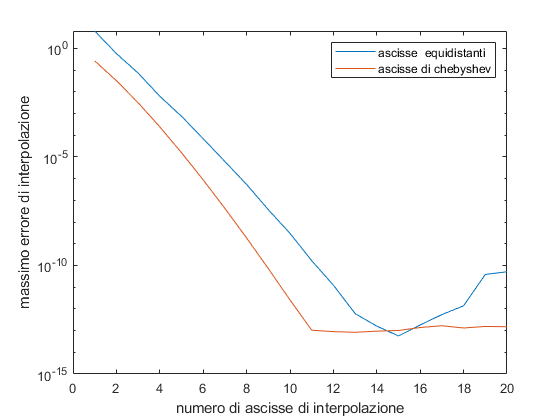
\includegraphics[scale=0.8]{capitolo4/hermite.png}
%     \caption{risultati interpolazione hermite}
%     \label{fig:16}
% \end{figure}


% Si può notare come, rispetto all'interpolazione classica, l'errore decresca più rapidamente per $n \le 15$. Anche in questo caso l'errore commesso usando le ascisse di chebyshev
% è migliore in confronto al caso delle ascisse equidistanti(eccetto per $n=15$).